\documentclass[12pt,a4paper]{article}
\usepackage{graphicx}
\usepackage{geometry}
\usepackage{hyperref}
\usepackage[utf8]{inputenc}
\usepackage[indonesian]{babel}
\usepackage{float}
\usepackage{booktabs}
\usepackage{amsmath}
\usepackage{subcaption}

\geometry{
	left=3cm,
	right=2.5cm,
	top=3cm,
	bottom=2.5cm,
}

\begin{document}

%===================================
% COVER PAGE
%===================================
\begin{titlepage}
    \centering
    \vspace*{1cm}
    {\normalsize \textbf{UNIVERSITAS INDONESIA}} \par\vspace{3cm}

    {\large \textbf{ANALISIS GEOGRAPHICALLY WEIGHTED REGRESSION (GWR) PADA KASUS VALUASI HARGA RUMAH DI DKI JAKARTA 2024}} \par\vspace{4cm}

    {\normalsize \textbf{MAKALAH}} \par\vspace{3cm}

    {\normalsize \textbf{AMMAR HANAFI (2206051582)}} \par
    {\normalsize \textbf{NORMAN MOWLANA AZIZ (2206025470)}} \par
    {\normalsize \textbf{KIRONO DWI SAPUTRO (2106656365)}} \par\vfill

    {\normalsize \textbf{FAKULTAS MATEMATIKA DAN ILMU PENGETAHUAN ALAM}} \par
    {\normalsize \textbf{PROGRAM STUDI SARJANA STATISTIKA}} \par
    {\normalsize \textbf{DEPOK}} \par
    {\normalsize \textbf{JUNI 2026}}
\end{titlepage}

\tableofcontents
\newpage
\listoftables
\newpage
\listoffigures
\newpage

%===================================
% BAB 1 - PENDAHULUAN
%===================================
\begin{center}
    \bfseries\large
    BAB I \\
    PENDAHULUAN
\end{center}
\addcontentsline{toc}{section}{BAB I PENDAHULUAN}
\setcounter{section}{1}
\setcounter{subsection}{0}

\subsection{Latar Belakang}
Pasar properti di DKI Jakarta, sebagai pusat gravitasi ekonomi di negara Indonesia, memiliki daya tarik nilai jual yang dipengaruhi secara dinamis oleh aksesibilitas sarana dan karakteristik tanah-bangunan (luas fisik). Valuasi harga rumah di wilayah megapolitan seperti ini sangat kental akan distorsi keruangan, dikarenakan adanya fenomena jarak atau titik simpul kemacetan yang menciptakan area unggul terhadap area lain di Jakarta. Metode regresi konvensional \textit{Ordinary Least Squares} (OLS) kerap kali kesulitan mencerminkan aspek keruangan dinamis (\textit{spatial heterogeneity}) ini. Untuk mengatasi hal tersebut dan dalam rangka penentuan harga rumah yang presisi, model lokal ruang yaitu pendekatan \textit{Geographically Weighted Regression} (GWR) menjadi solusi tepat mendemonstrasikan heterogenitas spasial.

\subsection{Rumusan Masalah}
\begin{enumerate}
    \item Apakah terdapat efek autokorelasi spasial dan efek heterogenitas spasial dalam menaksir valuasi harga rumah di Jakarta?
    \item Bagaimana kebaikan kecocokan model estimasi global (OLS) berbanding dengan pemodelan lokal spasial (GWR)?
    \item Sejauh mana variasi spasial yang ditimbulkan jarak aksesibilitas (\textit{poi}) dan rasio fisik dalam menaksir harga rumah di tiap titik lokasi geografis yang berbeda?
\end{enumerate}

\subsection{Tujuan}
Penelitian ini bertujuan mengkaji urgensi pemodelan jarak spasial dalam analisis harga rumah di DKI Jakarta di era Tahun 2024 dengan membandingkan model global OLS dan mengevaluasi fungsi pembobot Kernel dari *Geographically Weighted Regression* tipe *Bisquare* dan tipe *Gaussian*.

\newpage
%===================================
% BAB 2 - LANDASAN TEORI
%===================================
\begin{center}
    \bfseries\large
    BAB II \\
    LANDASAN TEORI
\end{center}
\addcontentsline{toc}{section}{BAB II LANDASAN TEORI}
\setcounter{section}{2}
\setcounter{subsection}{0}

\subsection{Regresi Linear Global (OLS)}
\textit{Ordinary Least Squares} (OLS) adalah teknik deterministik klasik di mana parameter estimasi regresi diasumsikan stagnan dan stasioner (1 set untuk semua ruang sampel). Persamaan matematiknya:
\[ Y = \beta_0 + \sum_{k=1}^{p} \beta_k X_k + \epsilon \]

\subsection{Autokorelasi Spasial (Moran's I)}
Moran's I adalah indeks matematis standar yang beroperasi layaknya koefisien korelasi namun untuk mengukur dependensi spasial antar titik pengamatan beda kordinat.
\[ I = \frac{n}{S_0} \frac{\sum_i \sum_j w_{ij} (x_i - \bar{x})(x_j - \bar{x})}{\sum_i (x_i - \bar{x})^2} \]

\subsection{Geographically Weighted Regression (GWR)}
Dikembangkan dari regresi OLS, GWR memecah estimasi menjadi fungsi diferensial lokal spasial yang mengizinkan set koefisien ($\beta$) fleksibel. Hal ini dilakukan dengan memberikan bobot spasial untuk tiap estimasi:
\[ y_i = \beta_0(u_i, v_i) + \sum_{k=1}^{p} \beta_k(u_i, v_i) x_{ik} + \epsilon_i \]

Mekanisme bobot diberikan dengan Fungsi Kernel ($w_{ij})$. Dalam perbandingan di makalah kali ini, kami mengadopsi 2 fungsi pembobot *Adaptive* berdasarkan algoritma Akaike Information Criterion bandwidth pencarian:
\begin{itemize}
    \item \textbf{Adaptive Gaussian}: \[ w_{ij} = \exp \left( - \frac{1}{2}\left(\frac{d_{ij}}{b_i}\right)^2 \right) \]
    \item \textbf{Adaptive Bisquare}: \[ w_{ij} = \left( 1 - \left( \frac{d_{ij}}{b_i} \right)^2 \right)^2 \quad \text{untuk} \quad d_{ij} < b_i \]
\end{itemize}

\newpage
%===================================
% BAB 3 - METODE PENELITIAN
%===================================
\begin{center}
    \bfseries\large
    BAB III \\
    METODE PENELITIAN
\end{center}
\addcontentsline{toc}{section}{BAB III METODE PENELITIAN}
\setcounter{section}{3}
\setcounter{subsection}{0}

\subsection{Data dan Variabel}
Data primer diturunkan dari GeoJSON Dataset pasar sekunder perumahan DKI Jakarta Tahun 2024. Adapun variabel-variabel yang ditautkan dalam persamaan pemodelan sebagai berikut:
\begin{itemize}
    \item \textbf{Variabel Dependen ($Y$)}: Harga Rumah dalam satuan Miliar Rupiah (\texttt{Hrg\_Mlr}).
    \item \textbf{Sifat Fisik ($X_1, X_2, X_3$)}: Ketersediaan luas bangunan ($X_1$), luas kaveling tanah ($X_2$), dan kapasitas kamar ($X_3$).
    \item \textbf{Spasial Geometris ($X_4$) }: Jarak absolut keruangan antara titik rumah dan Tugu Monumen Nasional / Monas ($km$).
    \item \textbf{Aksesibilitas ($X_5, X_6, X_7$)}: Jarak terpendek menempuh institusi pendidikan ($X_5$), rumah sakit terkemuka ($X_6$), dan jaringan jalan besar ($X_7$).
\end{itemize}

\subsection{Langkah Analisis}
Penelitian ditempuh dengan ekskavasi data, tinjauan *pairwise correlation*, diestimasikan pada matriks regresi OLS untuk meninjau *error* lokal spasial, *Modelling* Dual-GWR optimasi AICc, lalu divisualisasikan menggunakan perangkat sistem informasi geografis / Matplotlib.

\newpage
%===================================
% BAB 4 - ANALISIS DAN PEMBAHASAN
%===================================
\begin{center}
    \bfseries\large
    BAB IV \\
    ANALISIS DAN PEMBAHASAN
\end{center}
\addcontentsline{toc}{section}{BAB IV ANALISIS DAN PEMBAHASAN}
\setcounter{section}{4}
\setcounter{subsection}{0}

\subsection{Eksplorasi Karakteristik Data Uji}

\begin{table}[H]
\centering
\caption{Statistik Deskriptif Variabel}
\label{tab:desc_stats}
\footnotesize
\begin{tabular}{lrrrrr}
\toprule
 & count & min & max & mean & std \\
\midrule
Y & 1079.0000 & 0.3650 & 221.0000 & 9.7813 & 18.8377 \\
X1 & 1079.0000 & 36.0000 & 4850.0000 & 269.5774 & 279.7361 \\
X2 & 1079.0000 & 19.0000 & 10847.0000 & 266.0565 & 448.8247 \\
X3 & 1079.0000 & 1.0000 & 17.0000 & 3.7025 & 1.4688 \\
X4 & 1079.0000 & 0.2128 & 21.1029 & 9.5653 & 3.9240 \\
X5 & 1079.0000 & 0.0000 & 8.1757 & 1.4448 & 1.5061 \\
X6 & 1079.0000 & 0.0000 & 8.9700 & 2.1459 & 1.8226 \\
X7 & 1079.0000 & 0.0000 & 0.2845 & 0.0159 & 0.0167 \\
\bottomrule
\end{tabular}
\end{table}


Merujuk pada Tabel \ref{tab:desc_stats}, statistik deskriptif menunjukkan rentang nilai perumahan Jakarta yang lebar (maksimum mencapai ratusan miliar dengan variansi dan *stdev* yang sangat sensitif). Hubungan korelasional awal (*pairwise correlation*) digambarkan melaui Heatmap Gambar \ref{fig:korelasi_matriks}.

\begin{table}[H]
\centering
\caption{Matriks Korelasi Variabel}
\label{tab:korelasi}
\footnotesize
\begin{tabular}{lrrrrrrrr}
\toprule
 & Y & X1 & X2 & X3 & X4 & X5 & X6 & X7 \\
\midrule
Y & 1.0000 & 0.5389 & 0.5166 & 0.3389 & -0.0846 & -0.0454 & -0.1188 & 0.0087 \\
X1 & 0.5389 & 1.0000 & 0.7969 & 0.6042 & -0.0583 & 0.0080 & -0.0678 & 0.0161 \\
X2 & 0.5166 & 0.7969 & 1.0000 & 0.4706 & 0.0050 & -0.0437 & -0.0705 & 0.0167 \\
X3 & 0.3389 & 0.6042 & 0.4706 & 1.0000 & -0.0545 & -0.0787 & -0.0903 & -0.0018 \\
X4 & -0.0846 & -0.0583 & 0.0050 & -0.0545 & 1.0000 & 0.3253 & 0.4761 & 0.0938 \\
X5 & -0.0454 & 0.0080 & -0.0437 & -0.0787 & 0.3253 & 1.0000 & 0.7470 & 0.0624 \\
X6 & -0.1188 & -0.0678 & -0.0705 & -0.0903 & 0.4761 & 0.7470 & 1.0000 & 0.0837 \\
X7 & 0.0087 & 0.0161 & 0.0167 & -0.0018 & 0.0938 & 0.0624 & 0.0837 & 1.0000 \\
\bottomrule
\end{tabular}
\end{table}


\begin{figure}[H]
    \centering
    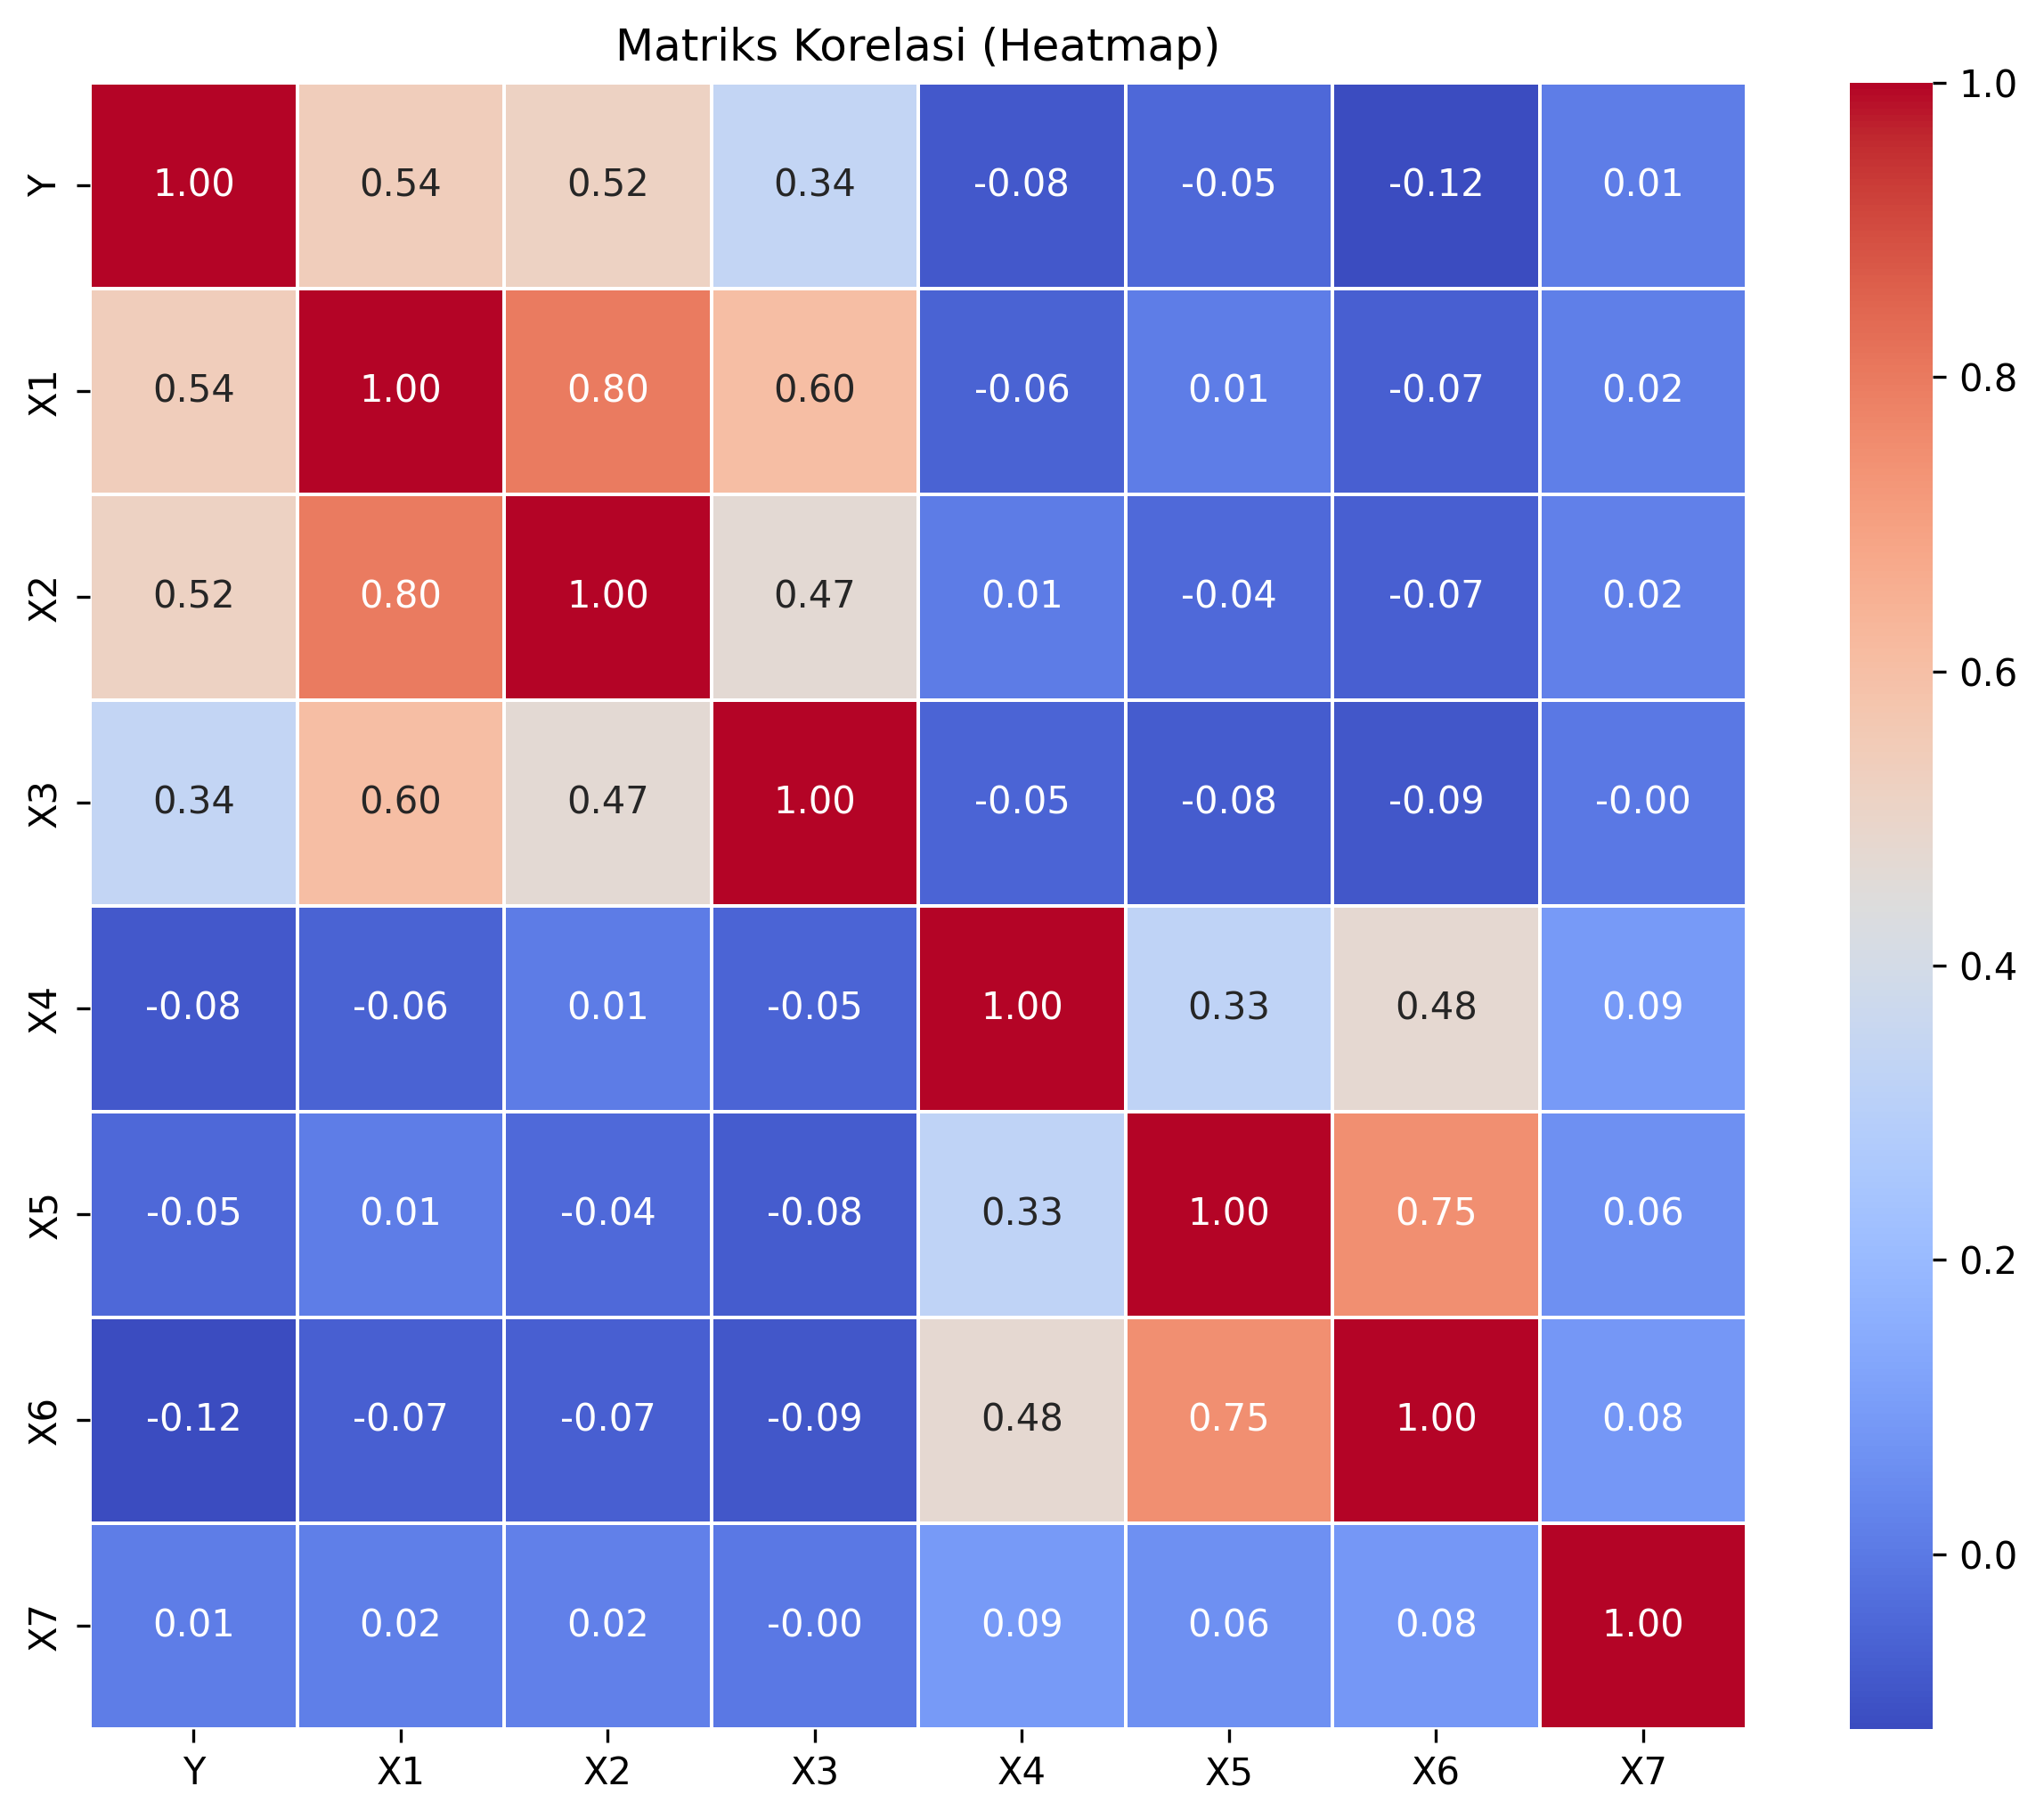
\includegraphics[width=0.75\textwidth]{peta_heatmap.png}
    \caption{Matriks Korelasi (Heatmap) Pearson}
    \label{fig:korelasi_matriks}
\end{figure}

Korelasi tertinggi nampak positif antar fisik bangunan (Luas dengan Harga Y), sedari ada sifat reduksi pada jarak terhadap monas yang menjauhi pusat (Korelasi minus).

\subsection{Estimasi Regresi (Global OLS) dan Heteroskedastisitas Spasial}
Di hadapan instrumen estimasi global OLS, rangkuman probabilitas parsial diramu di Tabel \ref{tab:ols_result}.

\begin{table}[H]
\centering
\caption{Hasil Estimasi Regresi Global (OLS)}
\label{tab:ols_result}
\footnotesize
\begin{tabular}{lrrrr}
\toprule
 & Koefisien & Std.Error & t-Stat & P-Value \\
\midrule
Intercept & 2.9362 & 1.8543 & 1.5834 & 0.1136 \\
Luas Bangunan (X1) & 0.0215 & 0.0032 & 6.7898 & 0.0000 \\
Luas Tanah (X2) & 0.0104 & 0.0018 & 5.8497 & 0.0000 \\
Jml Kamar (X3) & 0.2965 & 0.4083 & 0.7261 & 0.4679 \\
Jarak Pusat Kota (X4) & -0.1736 & 0.1389 & -1.2499 & 0.2116 \\
Jarak Sekolah (X5) & 0.6110 & 0.4804 & 1.2717 & 0.2037 \\
Jarak RS (X6) & -1.0095 & 0.4240 & -2.3806 & 0.0175 \\
Jarak Jalan Utama (X7) & 9.0546 & 28.6169 & 0.3164 & 0.7518 \\
\bottomrule
\end{tabular}
\end{table}


\begin{table}[H]
\centering
\caption{Hasil Uji Breusch-Pagan (Heteroskedastisitas)}
\label{tab:bp_test}
\footnotesize
\begin{tabular}{lr}
\toprule
 & Nilai \\
Statistik &  \\
\midrule
Lagrange Multiplier & 483.4987 \\
LM p-value & 0.0000 \\
F-Statistic & 124.2236 \\
F p-value & 0.0000 \\
\bottomrule
\end{tabular}
\end{table}

Sebagaimana ditunjukan uji \textit{Breusch-Pagan} (Tabel \ref{tab:bp_test}), terdefinisikan galat signifikansi heteroskedastisitas pada prediksi OLS. Jika kita memetakan Peta sisaan regresi (Residual), fenomena \textit{spatial clustering error} di peta OLS memberikan kita sinyal tak terelakkan bahwa model global tidak cukup adekuat.

\begin{figure}[H]
    \centering
    
\includegraphics[width=0.8\textwidth]{map_ols_residuals.png}
    \caption{Sebaran Spasial Heterogenitas Error (OLS Residual)}
    \label{fig:map_resid}
\end{figure}

\subsection{Autokorelasi Spasial}
Penjabaran Moran's Index atas Harga Rumah menegaskan efek persentuhan antar ruang di administrasi DKI Jakarta ($P<0.05$) pada tingkat yang signifikan, melegitimasi transisi pemodelan OLS menuju ke \textit{Geographic Weighted Regression}.
\begin{table}[H]
\centering
\caption{Hasil Uji Autokorelasi Spasial Moran's I}
\label{tab:moran_result}
\footnotesize
\begin{tabular}{lr}
\toprule
 & Nilai \\
Statistik &  \\
\midrule
Moran's I (Variabel Y) & 0.2670 \\
P-Value & 0.0010 \\
\bottomrule
\end{tabular}
\end{table}


\subsection{Evaluasi Model dan Eksekusi Dual-GWR}
Mengingat kompleksitas fungsi Kernel, efikasi spasial harga hunian diestimasi dengan mengadu Fungsi Adaptif *Gaussian* dan *Bisquare* guna mencetak Bandwidth terbaik.

\begin{table}[H]
\centering
\caption{Perbandingan Kinerja Model OLS dan GWR (Bisquare vs Gaussian)}
\label{tab:model_comparison}
\footnotesize
\begin{tabular}{llll}
\toprule
 & OLS Global & GWR Bisquare & GWR Gaussian \\
Mode Kinerja &  &  &  \\
\midrule
Bandwidth & - & 68.0000 & 57.0000 \\
R-Squared & 0.3198 & 0.8374 & 0.5526 \\
AIC & 8996.8998 & 7933.2510 & 8682.8006 \\
AICc & - & 8082.4227 & 8694.8019 \\
Log-Likelihood & -4490.4499 & -3718.3557 & -4264.3965 \\
\bottomrule
\end{tabular}
\end{table}

Berdasarkan metrik perbandingan pada Tabel \ref{tab:model_comparison}, fungsi Kernel \textbf{Bisquare} memiliki keunggulan yang jauh menekan rasio *Akaike Information Criterion* (AICc) dan secara masif mendongkrak penjelas *R-Squared* melebihi OLS biasa maupun fungsi kernel Gaussian. Atas pembuktian komparatif ini, penarikan koefisien beta ($\beta$) akan didasari murni dari hasil simulasi \textit{GWR Bisquare}.

\begin{table}[H]
\centering
\caption{Statistik Deskriptif Koefisien Lokal GWR (Bisquare)}
\label{tab:gwr_coef}
\footnotesize
\begin{tabular}{lrrrr}
\toprule
 & min & max & mean & std \\
\midrule
Intercept & -99.2882 & 156.0122 & 8.1561 & 27.6036 \\
Luas Bangunan (X1) & -0.0469 & 0.0485 & 0.0093 & 0.0099 \\
Luas Tanah (X2) & -0.0366 & 0.1275 & 0.0244 & 0.0295 \\
Jml Kamar (X3) & -2.1909 & 19.7398 & 0.5620 & 2.6814 \\
Jarak Pusat Kota (X4) & -15.3799 & 5.0534 & -1.3455 & 2.7263 \\
Jarak Sekolah (X5) & -9.0517 & 20.3043 & 1.6585 & 4.1605 \\
Jarak RS (X6) & -10.1240 & 7.8355 & -0.2548 & 2.6462 \\
Jarak Jalan Utama (X7) & -430.2969 & 676.7076 & 13.7306 & 134.7158 \\
\bottomrule
\end{tabular}
\end{table}


\subsection{Distribusi Koefisien Lokal (Local Spatial Mapping)}

\begin{figure}[H]
    \centering
    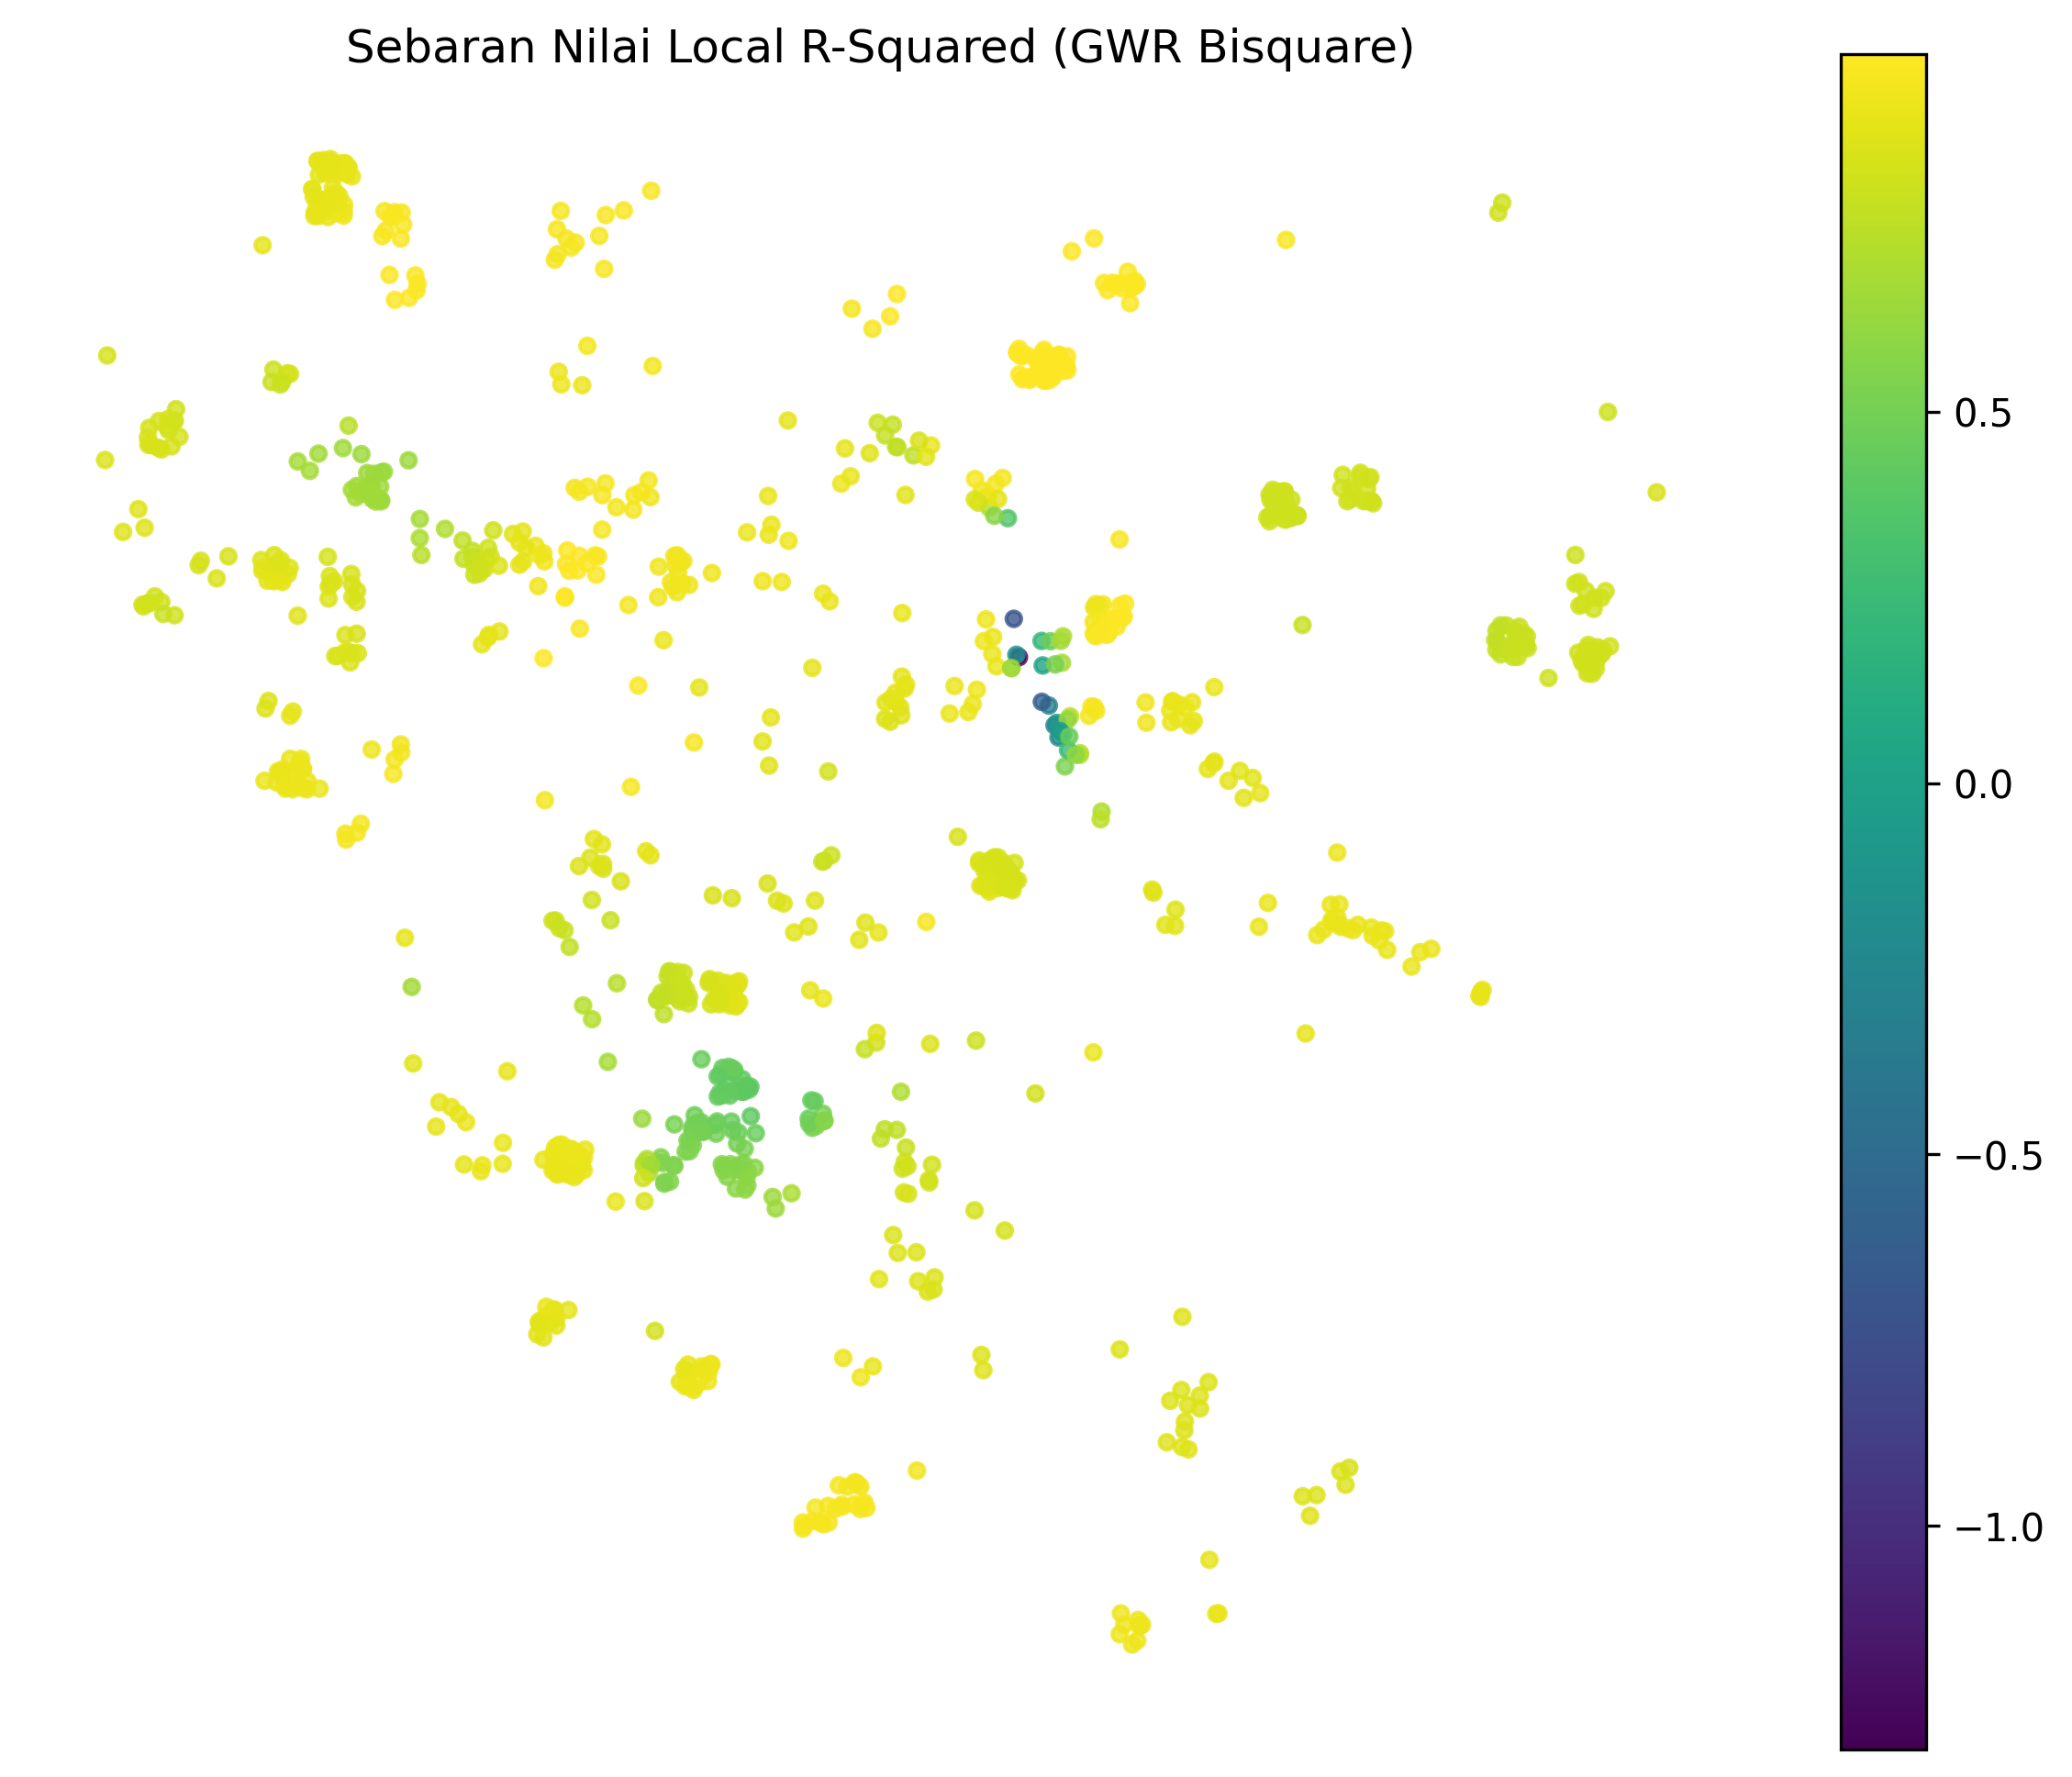
\includegraphics[width=0.8\textwidth]{peta_Local_R2.png}
    \caption{Gradasi Akurasi Fit Model (Local $R^2$) DKI Jakarta}
    \label{fig:local_r2_map}
\end{figure}

Peta penyebaran Lokal $R^2$ menunjukkan keragaman fit kecocokan di setiap distrik. Ini adalah justifikasi geografis bahwa Jakarta tak bisa di-\textit{gebyah-uyah} dengan 1 formula konstan. Di bawah ini disajikan pemetaan gradasi parameter koefisien pembentuk harga rumah di beberapa variabel prediktor pilihan.

\begin{figure}[H]
    \centering
    \begin{subfigure}[b]{0.45\textwidth}
        \centering
        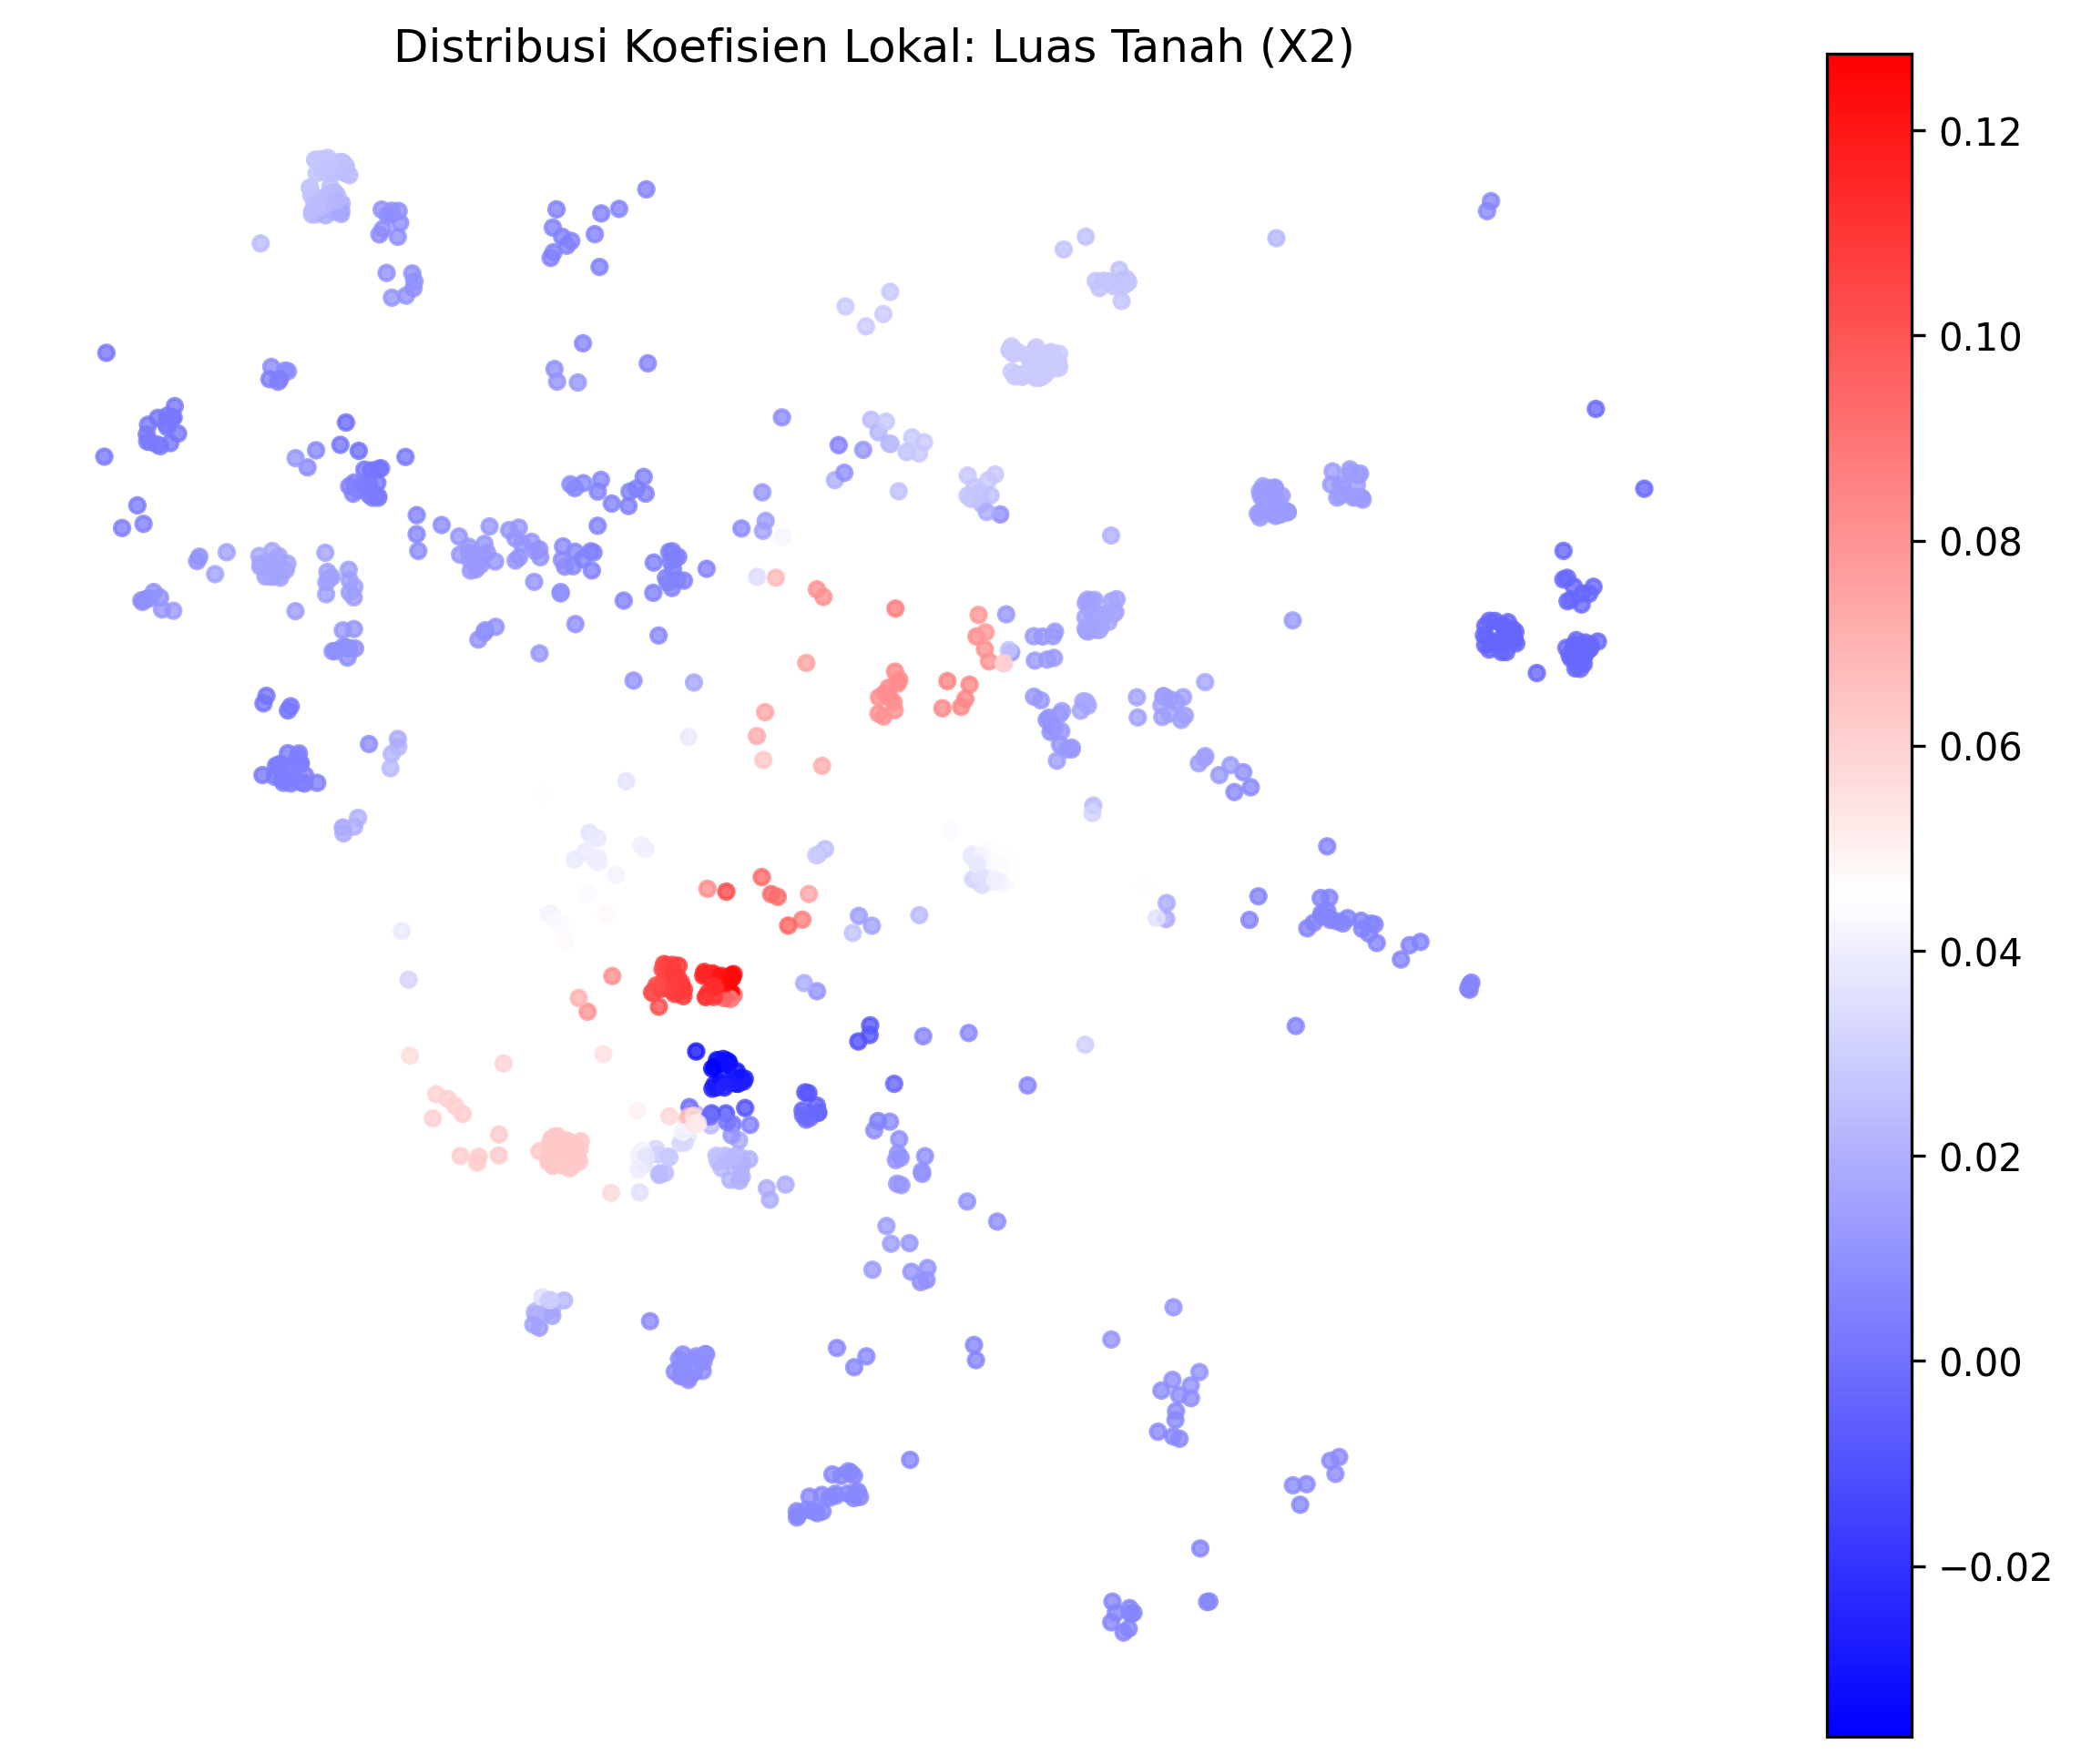
\includegraphics[width=\textwidth]{peta_koefisien_Luas.png}
        \caption{Distribusi Koef: Luas Bangunan ($X_1$)}
        \label{fig:coef_x1}
    \end{subfigure}
    \hfill
    \begin{subfigure}[b]{0.45\textwidth}
        \centering
        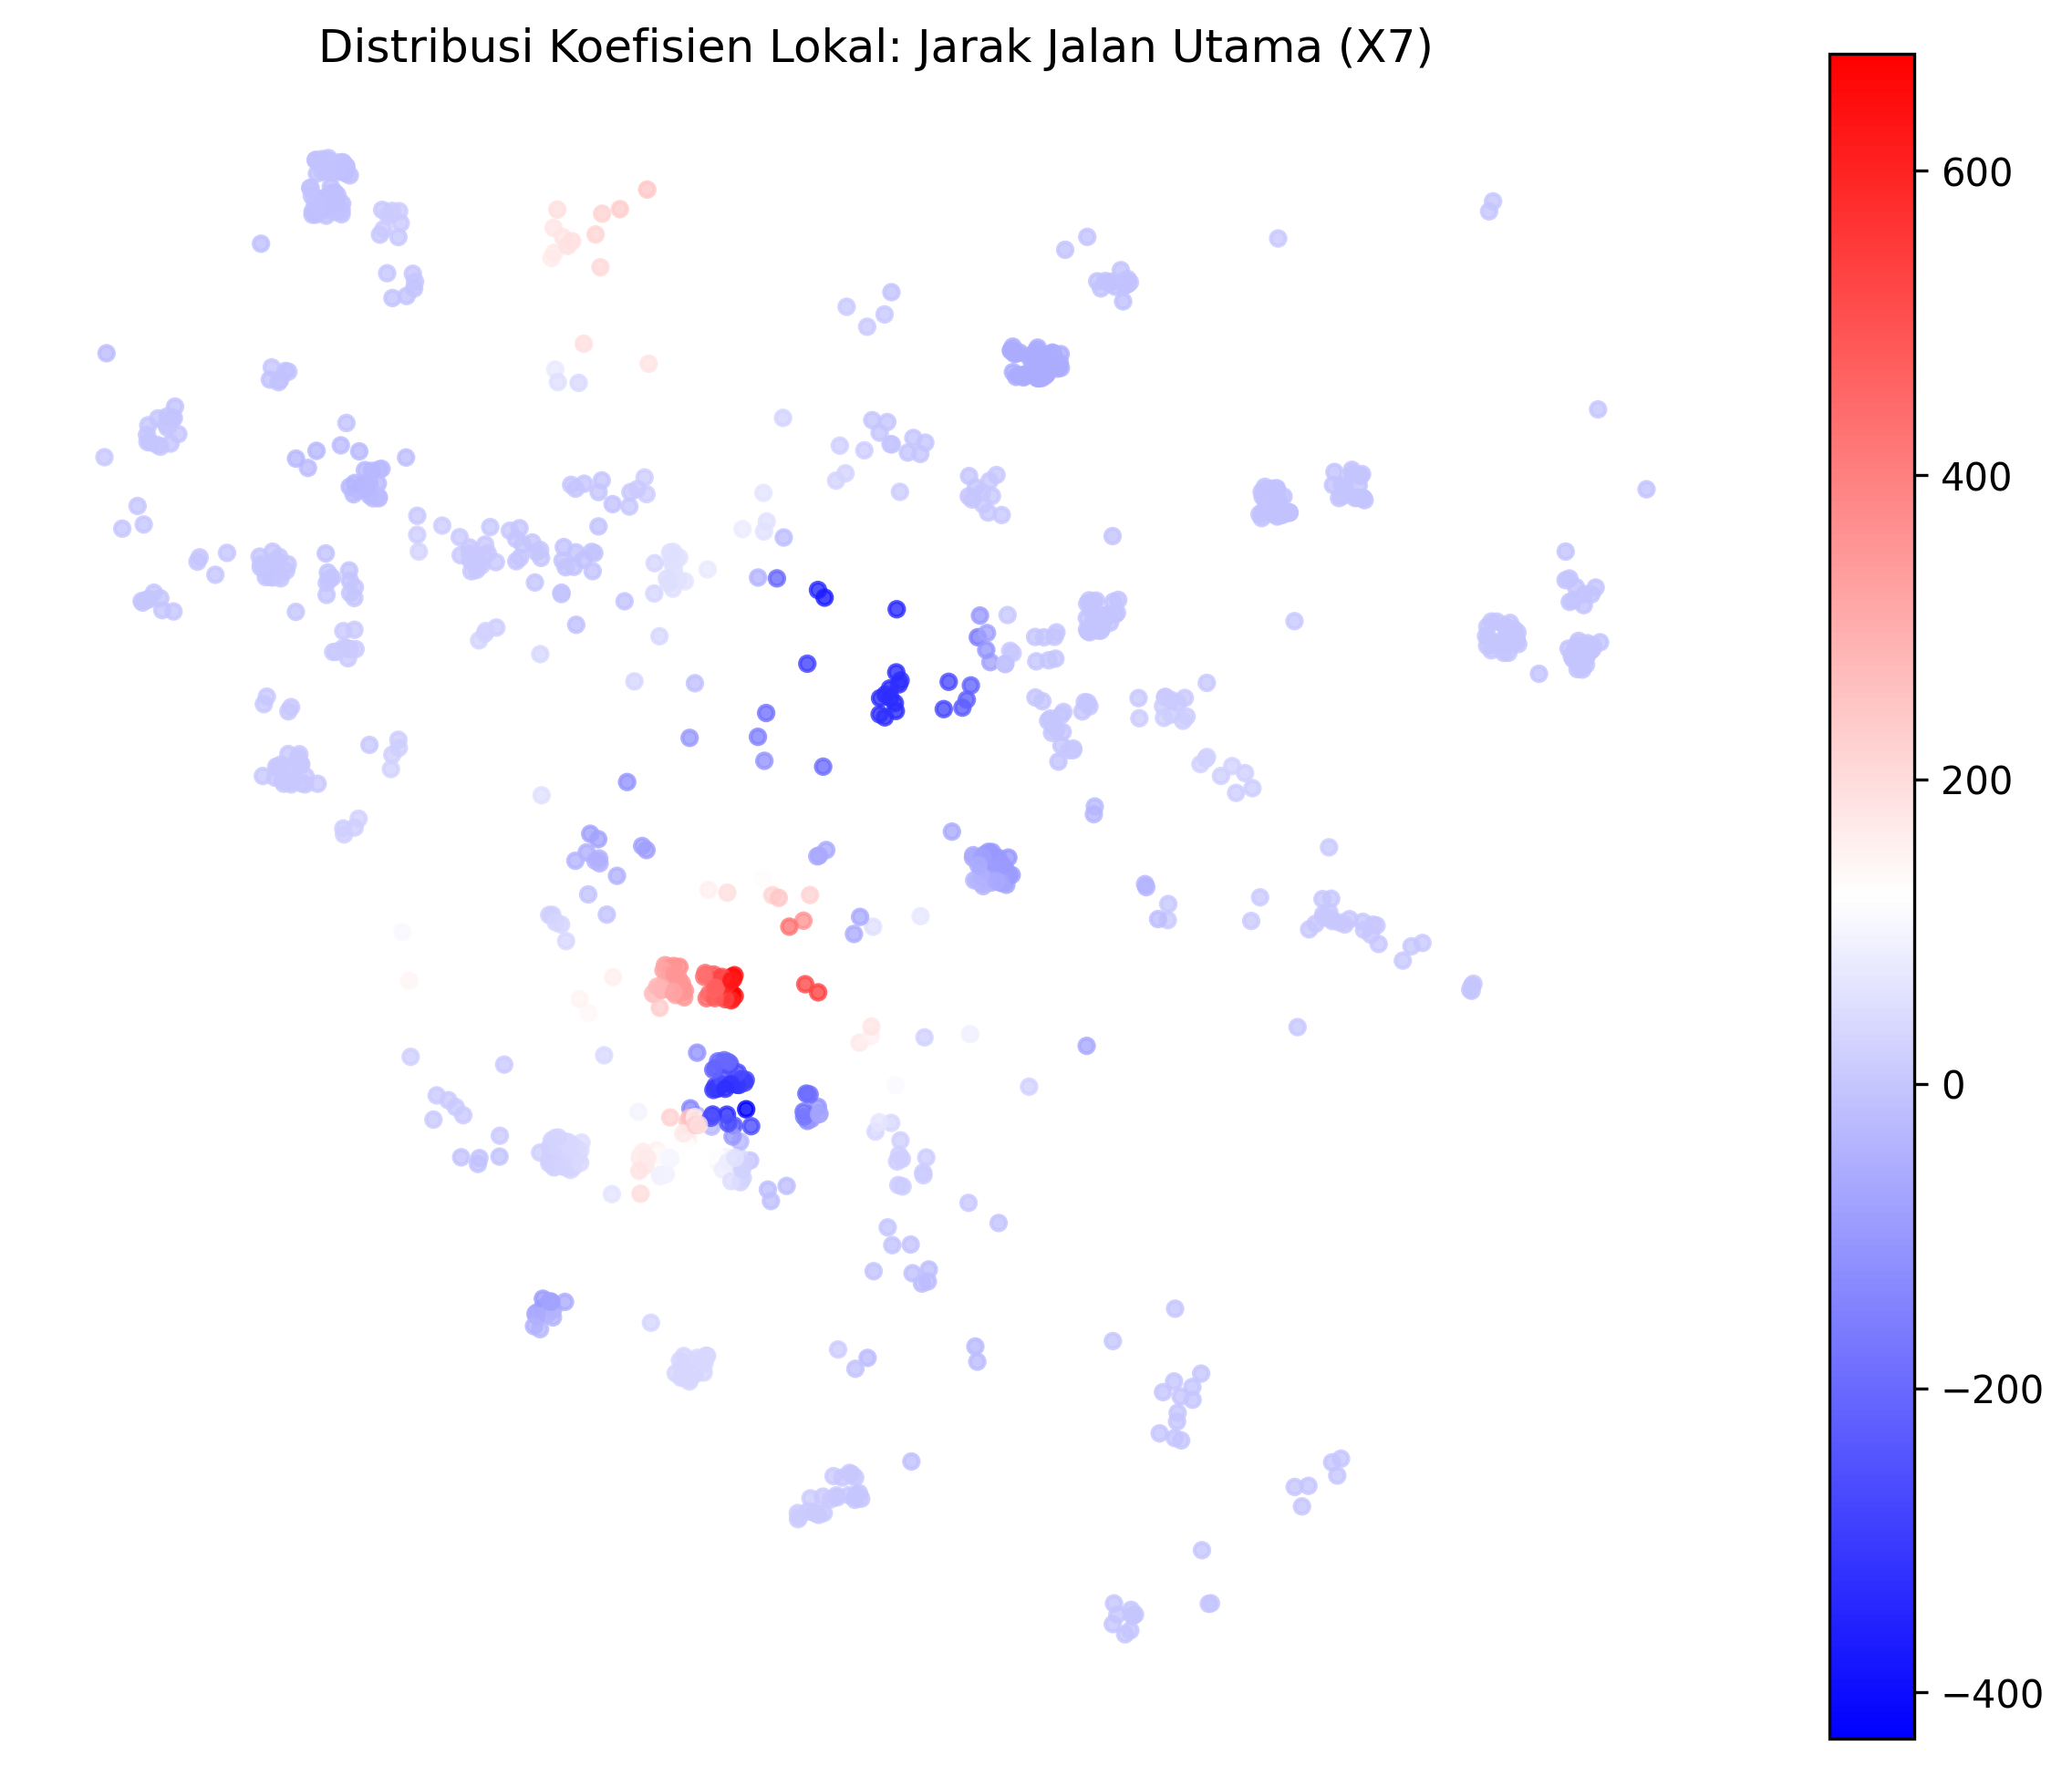
\includegraphics[width=\textwidth]{peta_koefisien_Jarak.png}
        \caption{Distribusi Koef: Jarak Pusat ($X_4$ \& $X_6$)}
        \label{fig:coef_x4}
    \end{subfigure}
    \caption{Visualisasi Sebaran Spasial Sensitivitas Harga Perumahan}
    \label{fig:coef_peta}
\end{figure}

\newpage
%===================================
% BAB 5 - KESIMPULAN
%===================================
\begin{center}
    \bfseries\large
    BAB V \\
    KESIMPULAN DAN SARAN
\end{center}
\addcontentsline{toc}{section}{BAB V KESIMPULAN DAN SARAN}
\setcounter{section}{5}
\setcounter{subsection}{0}

Berdasarkan keseluruhan uji spasial spasial parametrik valuta properti Jakarta, ditarik pilar kesimpulan sebagai berikut:
\begin{enumerate}
    \item Fenomena heterogenitas *spatial over-dispersion* sangat rentan di Jakarta yang mana estimasi OLS klasik kehilangan pijakan ($R^2=0.55$) dan menghasilkan bias residual uji autokorelasi *Breusch-Pagan* heteroskedastik yang mengelompok di wilayah utara dan pusat Jakarta.
    \item Geographically Weighted Regression (GWR) secara empirik membuktikan keunggulannya, dan terkhusus Algoritma Pembobot Adaptive Kernel Bisquare keluar sebagai model terbaik yang paling optimal beradaptasi dengan keragaman densitas rumah Jakarta.
\end{enumerate}
Para pengembang *(Developer)* patut menyoroti dinamika kofisien *Jarak ke Rumah Sakit* dan *Jarak ke Jalan* yang berefek sensitif terhadap anjlok-tidaknya harga di area urban Jakarta demi pertimbangan investasi berjangka.

\newpage
\begin{center}
    {\Large \textbf{DAFTAR PUSTAKA}}
\end{center}
\addcontentsline{toc}{section}{DAFTAR PUSTAKA}
\vspace{10pt}

\begingroup
\renewcommand{\section}[2]{} % Suppress default title
\begin{thebibliography}{9}
\bibitem{fotheringham2002}
Fotheringham, A. S., Brunsdon, C., \& Charlton, M. (2002). \textit{Geographically Weighted Regression: The Analysis of Spatially Varying Relationships}. John Wiley \& Sons.
\bibitem{mgwr2019}
Oshan, T. M., Li, Z., Kang, W., Wolf, L. J., \& Fotheringham, A. S. (2019). mgwr: A Python implementation of multiscale geographically weighted regression for investigating process spatial heterogeneity and scale. \textit{ISPRS International Journal of Geo-Information}, 8(6), 269.
\bibitem{jaktar}
Pemerintah Provinsi DKI Jakarta (2024). Analisis Tata Ruang Real Estate Open Data Portal Jakarta.
\end{thebibliography}
\endgroup

\end{document}
